%%%%%%%%%%%%%%%%%%%%%%%%%%%%%%%%%%%%%%%%%%%%%%%%%%%%%%%%%%%%%%%%%%%%%%%%%%%%%%%%%%%%%%%%%%%%%%%%
%
% CS484 Written Question Template
%
% Acknowledgements:
% The original code is written by Prof. James Tompkin (james_tompkin@brown.edu).
% The second version is revised by Prof. Min H. Kim (minhkim@kaist.ac.kr).
%
% This is a LaTeX document. LaTeX is a markup language for producing 
% documents. Your task is to fill out this document, then to compile 
% it into a PDF document. 
%
% 
% TO COMPILE:
% > pdflatex thisfile.tex
%
% If you do not have LaTeX and need a LaTeX distribution:
% - Personal laptops (all common OS): www.latex-project.org/get/
% - We recommend latex compiler miktex (https://miktex.org/) for windows,
%   macTex (http://www.tug.org/mactex/) for macOS users.
%   And TeXstudio(http://www.texstudio.org/) for latex editor.
%   You should install both compiler and editor for editing latex.
%   The another option is Overleaf (https://www.overleaf.com/) which is 
%   an online latex editor.
%
% If you need help with LaTeX, please come to office hours. 
% Or, there is plenty of help online:
% https://en.wikibooks.org/wiki/LaTeX
%
% Good luck!
% Min and the CS484 staff
%
%%%%%%%%%%%%%%%%%%%%%%%%%%%%%%%%%%%%%%%%%%%%%%%%%%%%%%%%%%%%%%%%%%%%%%%%%%%%%%%%%%%%%%%%%%%%%%%%
%
% How to include two graphics on the same line:
% 
% \includegraphics[width=0.49\linewidth]{yourgraphic1.png}
% \includegraphics[width=0.49\linewidth]{yourgraphic2.png}
%
% How to include equations:
%
% \begin{equation}
% y = mx+c
% \end{equation}
% 
%%%%%%%%%%%%%%%%%%%%%%%%%%%%%%%%%%%%%%%%%%%%%%%%%%%%%%%%%%%%%%%%%%%%%%%%%%%%%%%%%%%%%%%%%%%%%%%%

\documentclass[11pt]{article}

\usepackage[english]{babel}
\usepackage[utf8]{inputenc}
\usepackage[colorlinks = true,
linkcolor = blue,
urlcolor  = blue]{hyperref}
\usepackage[a4paper,margin=1.5in]{geometry}
\usepackage{stackengine,graphicx}
\usepackage{fancyhdr}
\setlength{\headheight}{15pt}
\usepackage{microtype}
\usepackage{times}
\usepackage{amsmath}
\usepackage{amssymb}
\usepackage{graphicx}

% From https://ctan.org/pkg/matlab-prettifier
\usepackage[numbered,framed]{matlab-prettifier}

\frenchspacing
\setlength{\parindent}{0cm} % Default is 15pt.
\setlength{\parskip}{0.3cm plus1mm minus1mm}

\pagestyle{fancy}
\fancyhf{}
\lhead{Homework 2 Questions}
\rhead{CS484}
\rfoot{\thepage}

\date{}

\title{\vspace{-1cm}Homework 2 Questions}


\begin{document}
	\maketitle
	\vspace{-3cm}
	\thispagestyle{fancy}
	
	\section*{Instructions}
	\begin{itemize}
		\item 4 questions.
		\item Write code where appropriate.
		\item Feel free to include images or equations.
		\item Please make this document anonymous.
		\item \textbf{Please use only the space provided and keep the page breaks.} Please do not make new pages, nor remove pages. The document is a template to help grading.
		\item If you really need extra space, please use new pages at the end of the document and refer us to it in your answers.
	\end{itemize}

	\section*{Questions}
	
	\paragraph{Q1:} Explicitly describe image convolution: the input, the transformation, and the output. Why is it useful for computer vision?
	
	%%%%%%%%%%%%%%%%%%%%%%%%%%%%%%%%%%%
	\paragraph{A1:} In mathematical view, image convolution uses 2D matrix to effect the image. To achieve image convolution, we should receive an image, and the filter, usually has smaller size compared to the image.
	In transformation part, flipping the filter horizontally and vertically at first is necessary. Then locate the filter's first element at the pixel of the image. Do the elementwise multiplication, and sum up the result of the calculation, the output image's pixel at the same position of the center element of the filter would have that value.
	Do this for every pixel of the image. When filter exceeds the image, we need paddings for image to calculate the result properly. The padding could be 0, or the reflection of the image.
	After all the jobs are completed, the output image will come out, the image applied filter to the original image.
	
	We can extract the important information easily with the convolution.
	
	
	%%%%%%%%%%%%%%%%%%%%%%%%%%%%%%%%%%%
	
	% Please leave the pagebreak
	\pagebreak
	\paragraph{Q2:} What is the difference between convolution and correlation? Construct a scenario which produces a different output between both operations.
	
	\emph{Please use \href{https://www.mathworks.com/help/images/ref/imfilter.html}{$imfilter$} to experiment! Look at the `options' parameter in MATLAB Help to learn how to switch the underlying operation from correlation to convolution.}
	
	%%%%%%%%%%%%%%%%%%%%%%%%%%%%%%%%%%%
	\paragraph{A2:} Convolution does flipping filter horizontally and vertically before doing the elementwise operation while correlation doesn't. By doing this, convolution allows image to preserve the order of occurred changes. So the difference occurs when the filter is not symmetric.
	For example, using the matrix below as a kernel:

	\begin{equation*}
		\begin{bmatrix}
			-15 & 0 & 0 \\
			0 & 0 & 0 \\
			0 & 0 & 16
		\end{bmatrix}
	\end{equation*}
	
	Using convolution and correlation generates the images below.
	\begin{figure}[h]
		\centering
		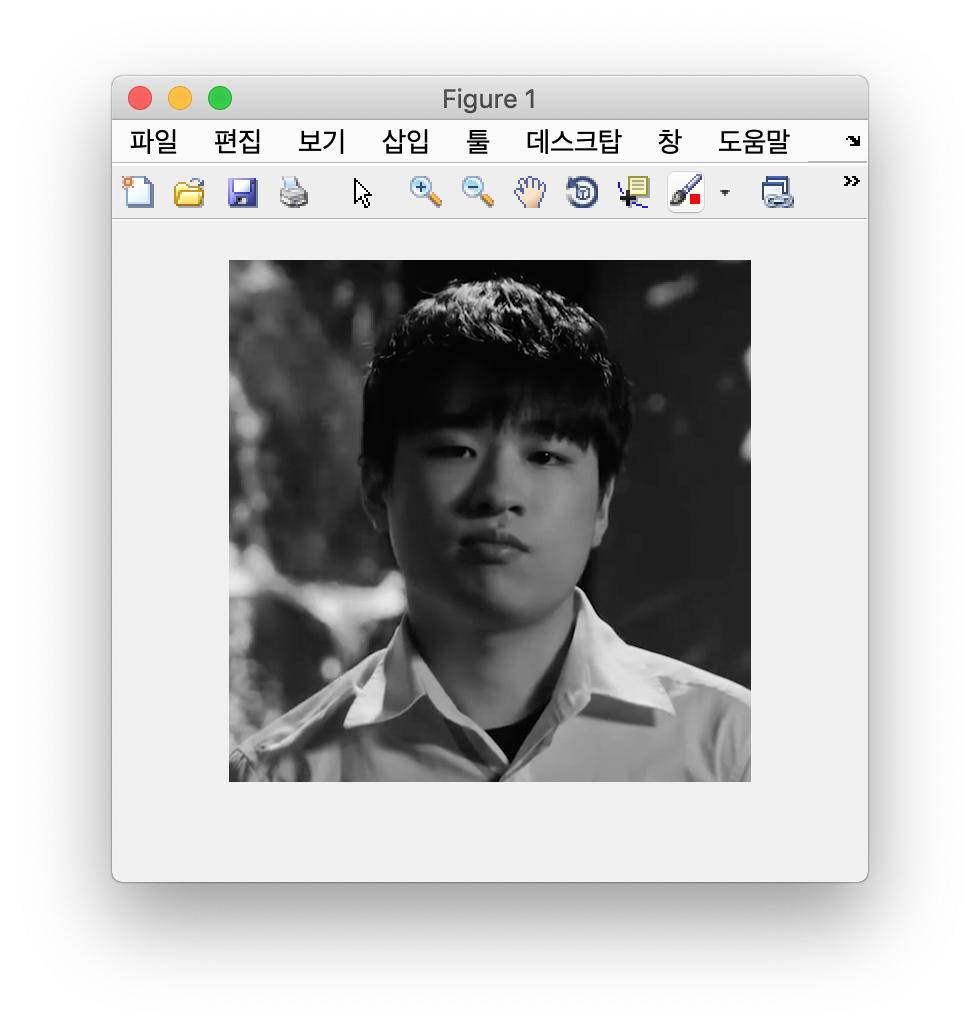
\includegraphics[width=5cm]{maru_origin.png}
		\caption{Original image}
		\label{fig:original image}
	\end{figure}

	\begin{figure}[h]
		\centering
		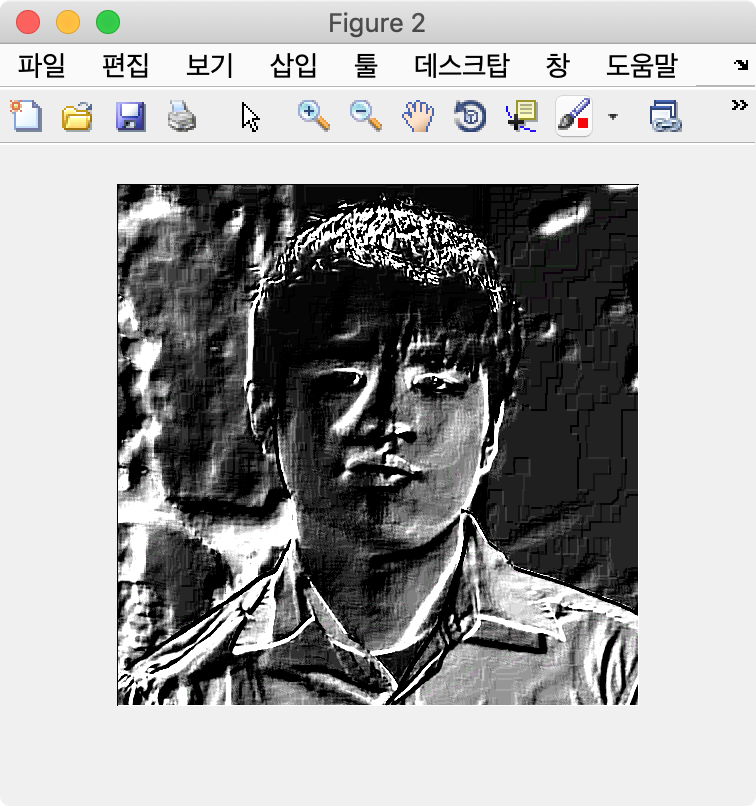
\includegraphics[width=5cm]{maru_conv.png}
		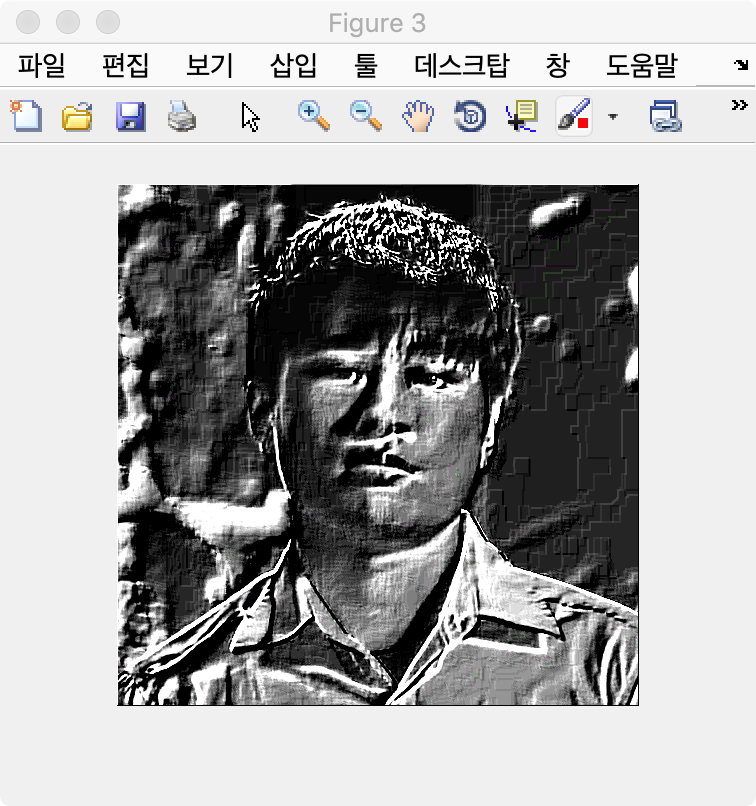
\includegraphics[width=5cm]{maru_corr.png}
		\caption{\emph{Left:} Image generated with convolution \emph{Right:} Image generated with correlation}
		\label{fig:convolution and correlation}
	\end{figure}
	%%%%%%%%%%%%%%%%%%%%%%%%%%%%%%%%%%%
	
	% Please leave the pagebreak
	\pagebreak
	\paragraph{Q3:} What is the difference between a high pass filter and a low pass filter in how they are constructed, and what they do to the image? Please provide example kernels and output images.
	
	%%%%%%%%%%%%%%%%%%%%%%%%%%%%%%%%%%%
	\paragraph{A3:} High pass filter is used for sharpening the image. For example, high pass filter uses kernels like
	\begin{equation*}
		\begin{bmatrix}
			0 & -1/4 & 0 \\
			-1/4 & 2 & -1/4 \\
			0 & -1/4 & 0
		\end{bmatrix}
	\end{equation*}
	this kernel emphasizes the difference between nearby pixels.
	
	In opposite, low pass filter is used for blurring the image. It looks like 
	\begin{equation*}
		\begin{bmatrix}
			1/9 & 1/9 & 1/9 \\
			1/9 & 1/9 & 1/9 \\
			1/9 & 1/9 & 1/9
		\end{bmatrix}
	\end{equation*}
	This makes the pixels' values similar to nearby pixels.

	And here are the images applied two filters.
	
	\begin{figure}[h]
		\centering
		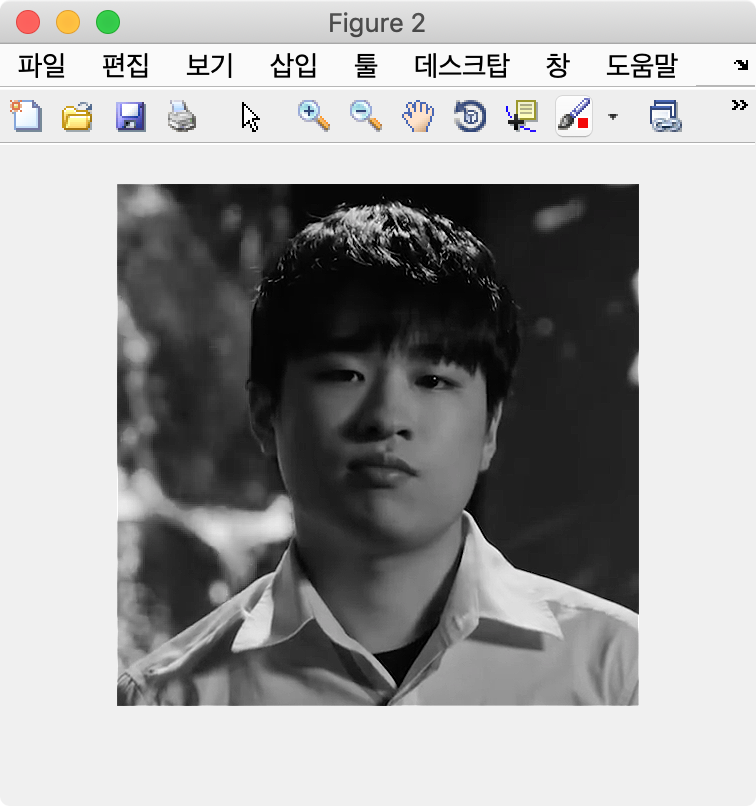
\includegraphics[width=5cm]{maru_high.png}
		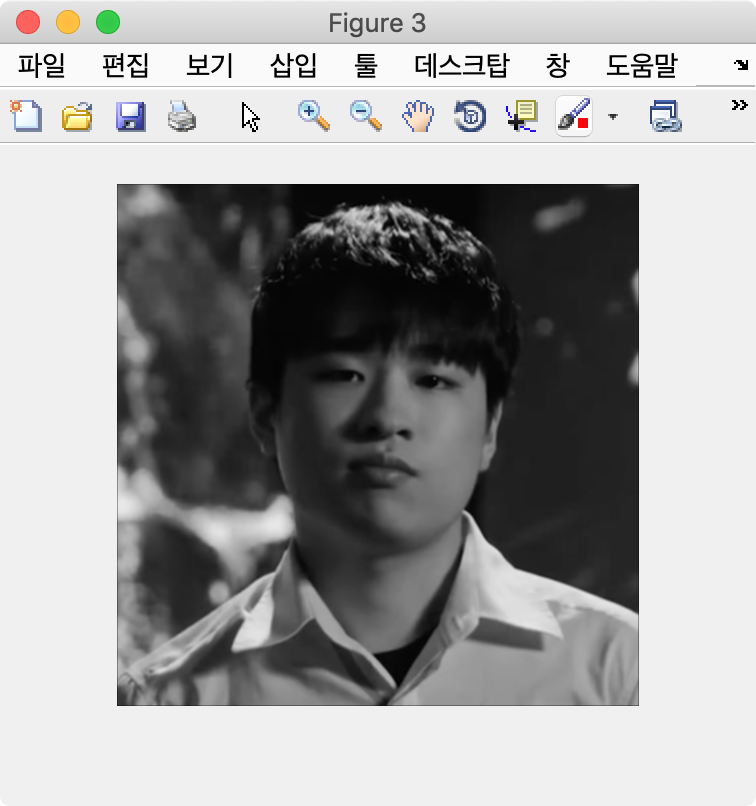
\includegraphics[width=5cm]{maru_low.png}
		\caption{\emph{Left:} High pass filter \emph{Right:} Low pass filter}
		\label{fig:high and low filter}
	\end{figure}
	
	%%%%%%%%%%%%%%%%%%%%%%%%%%%%%%%%%%%
	
	% Please leave the pagebreak
	\pagebreak
	\paragraph{Q4:} How does computation time vary with filter sizes from $3\times3$ to $15\times15$ (for all odd and square sizes), and with image sizes from 0.25~MPix to 8~MPix (choose your own intervals)? Measure both using \href{https://www.mathworks.com/help/images/ref/imfilter.html}{$imfilter$} to produce a matrix of values. Use the \href{https://www.mathworks.com/help/images/ref/imresize.html}{$imresize$} function to vary the size of an image. Use an appropriate charting function to plot your matrix of results, such as \href{https://www.mathworks.com/help/matlab/ref/scatter3.html}{$scatter3$} or \href{https://www.mathworks.com/help/matlab/ref/surf.html}{$surf$}.
	
	Do the results match your expectation given the number of multiply and add operations in convolution?
	
	See RISDance.jpg in the attached file.
	
	%%%%%%%%%%%%%%%%%%%%%%%%%%%%%%%%%%%
	\paragraph{A4:} If kernel size is [2m x 2n], it is expected to spend 4x time than the [m x n] kernel because it needs 4x multiplication operations.
	Also, if pixel number increases from N to 2N, it would take 2x time because we need to take 2x addition operations.
	However, here is the result:

	\begin{figure}[h]
		\centering
		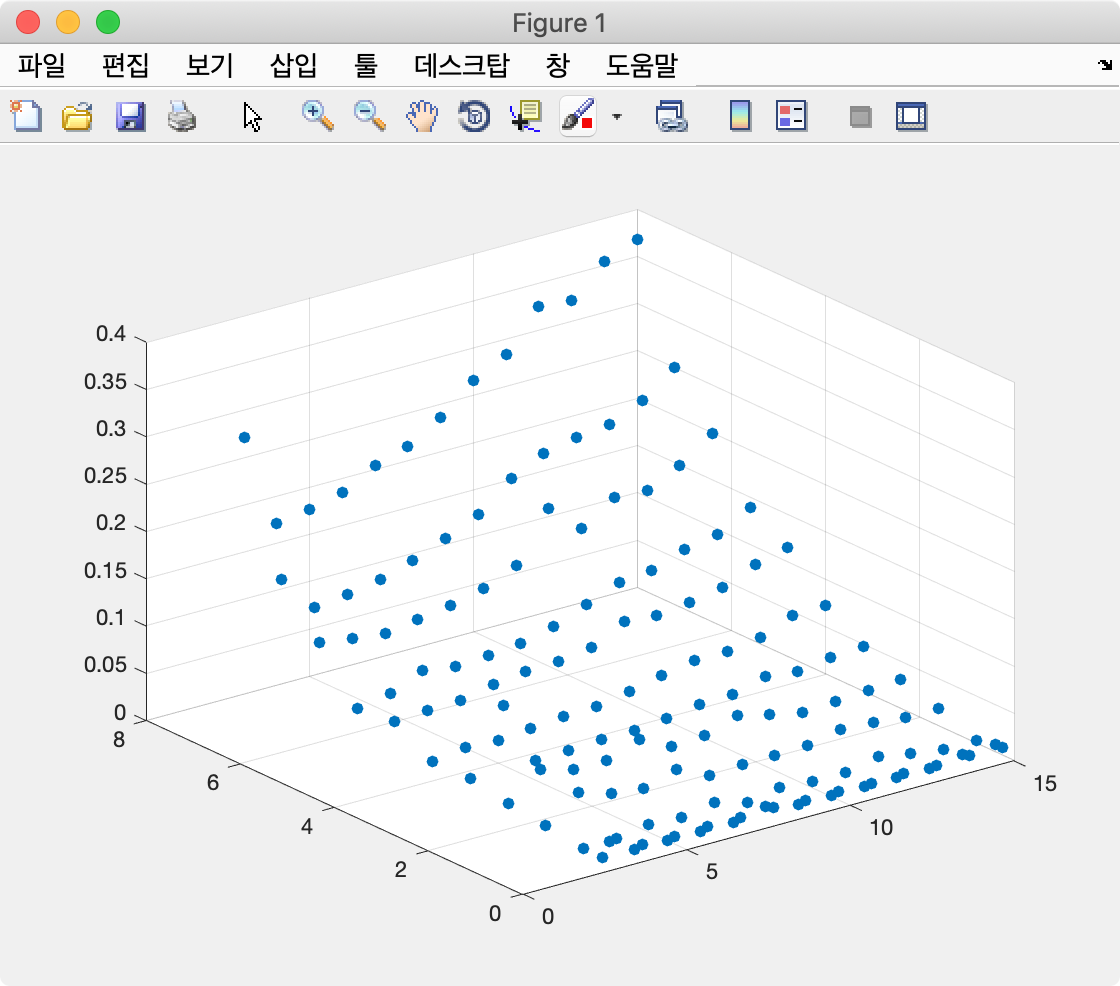
\includegraphics[width=7cm]{tictoc.png}
		\caption{Result of elapsed time}
		\label{fig:tic toc result}
	\end{figure}

	x-axis means kernel size, y-axis means pixel numbers, z-axis means elapsed time.
	It seems that kernel size is linear with elapsed time, and $(\text{pixel numbers})^2$ is linear with elapsed time. It is diffrent with expectation.
	
	
	
	%%%%%%%%%%%%%%%%%%%%%%%%%%%%%%%%%%%
	
	
	% If you really need extra space, uncomment here and use extra pages after the last question.
	% Please refer here in your original answer. Thanks!
	%\pagebreak
	%\paragraph{AX.X Continued:} Your answer continued here.
	
	
	
\end{document}